%MUHURTA  ADVANCED MATERIAL
 

%This lesson builds on the information given in the previous lesson. It is more technical and introduces a number of new astrological concepts. Hence, it may take more time and effort for the student. Again, much of it is advanced and supplementary in nature and it is not necessary for the student to grasp all of it before completing the course. Much of the information will be useful as a reference, therefore, the questions at the end of this lesson have been kept simple.

 

%We begin with an audio to explain the background of the Hindu lunar calendar and its five factors, what is called Panchanga, and the issues of its calculation and usage. This can be complex mainly owing to the variable movement of the Moon through the zodiac. Some variations are there as Panchangas are place specific, reflecting actual time starting with sunrise as the key factor of the day. These factors will be explained in more detail in the lesson.

\subsection{\textbf{Audio: The Panchanga or Vedic Astrological Calendar, its Importance and its Calculation}}

\subsection{II. TITHIS OR LUNAR DAYS}

After the Nakshatras as the first consideration which we discussed in the previous lesson, the Tithis are the most important factor of Muhurta. Tithis refer to the phases of the Moon and also roughly correspond to lunar days.

 

The Goddesses are closely related to the Phases of the Moon or Tithis

 


\subsubsection{THE SIXTEEN KALAS OF THE MOON}

Before we introduce the lunar days, we must first understand how Vedic thought views the Moon. This is important both for spiritual and ordinary actions.

 

In Vedic and Tantric thought, the Moon is said to contain sixteen portions or Kalas. The sixteenth Kala is unchangeable and represents the basic power or energy (shakti) of the Moon, through which it is able to continually renew itself in the cycles of time.

 

The number of the other Kalas increases and decreases with the waxing and waning of the Moon. On the day of the new Moon, the Moon is reduced to only one Kala, the immutable sixteenth. Then it gains one Kala every day approximately until reaching the full sixteen on the day of the full Moon.

 

The increasing and decreasing of the portions of the Moon shows our experience of karma, the cycle of enjoyment of the fruits of our action. It shows the fluctuations of the mind, as the Moon represents the mind or feeling nature in general.

 


\subsubsection{THE PURUSHA OR COSMIC PERSON}

In Vedic thought, the Purusha or cosmic person (time personified), the individual who is a microcosm of the universe, is said to consist of sixteen parts comprised of the following:

 

\begin{enumerate}
\item[*] The five elements: Earth, Water, Fire, Air, Ether
\item[*] The five organs of action: Reproductive organs, Organ of elimination, Organ of motion or feet, Hands, Vocal organ
\item[*] The five sense organs: Smell, Taste, Sight, Touch, Sound
 \end{enumerate}

Each organ of action and sense organ corresponds to one element respectively (ie. earth, the reproductive organs, and the organ of smell correspond). The Purusha, or mind, is the sixteenth factor, through which all the other fifteen are correlated. This is all part of standard Hindu philosophy and cosmology deriving from the Sankhya system.

 

Thus, the Purusha in its manifestation reflects the movement of the Moon. On the first five days after the new Moon, the five elements are formed which have an inert or tamasic nature. On the second five days, the corresponding five organs of action are formed, which have an active or rajasic nature. On the third five days, the corresponding five sense organs are formed, which have a pure or sattvic nature.

 

During the five days after the full Moon, the five sense organs get withdrawn. On the second five days, the five organs of action get withdrawn. On the third five days, the five elements get withdrawn. In the individual, however, these fluctuations are minor, although still important.

 

By mastering these energies through meditation, we gain the energy of bliss. By being dominated by them through the senses, we end up in sorrow and exhaustion. In this way, the portions of the Moon give us a key to our entire spiritual development. Yet they also can be used for ordinary actions and for understanding our monthly fluctuations of energy.

 

\subsubsection{TITHIS DEFINED}

In Vedic Astrology, the period between two full Moons, or a lunar month, is divided into thirty lunar days called “Tithis” which measure the Kalas or portions of the Moon. The Tithis are next to the Nakshatras in importance and are related to them.

 

The period between two full moons is about 29½ days, or a little shorter than a regular month of thirty or thirty-one days. Each lunar day or Tithi averages a little shorter than one day. To be exact, each Tithi marks an average period of 23 hours and 37 minutes, or about 23 minutes short of a regular day. There are thus 371 Tithis in a normal year of 365 days.

 

The Tithis, however, are irregular in length. They are calculated according to 12- degree movements between the Sun and Moon (with the Sun moving about 1 degree per day versus the 13-degree movement of the Moon), or according to the phases of the Moon. The Moons rate of motion is irregular. It varies from 11 to 15 degrees a day. This means that an actual Tithi may be a little longer or shorter than a day. Hence, Tithis require an almanac for their calculation. The Tithi for the day is determined by the Tithi in effect at sunrise. When the Moons rate of motion is fast, there may be two Tithis in one day. A Tithi may therefore be skipped in the calendar (called a “kshaya tithi” in the Panchanga). When the Moons rate is slow, which is more rare, the same Tithi may occur on two consecutive days (an increased or “vriddha” tithi). Always go back to the Tithi of the previous dawn for determining what Tithi is in effect at any time during the day for horary astrology or Prashna. For natal astrology, you can use the Tithi in operation at the birth time.

 

There are 15 types of Tithis, divided into two groups relative to the waxing and waning Moon, creating a total of 30. The bright or waxing half of the Moon is called Shukla Paksha (also known as Sita Paksha). The 15 Tithis of Shukla Paksha extend from the new Moon at the beginning of the first Tithi, to the full Moon at the end of the fifteenth Tithi. The dark or waning half of the Moons phase is called Krishna Paksha. The 15 Tithis of Krishna Paksha extend from the full Moon at the beginning of the first Tithi, to the new Moon at the end of the fifteenth Tithi.

 

This means that in Vedic Astrology there are really two days of the full Moon and two days of the new Moon. Purnima ends with the Moon becoming exactly full. Hence, it refers to the lunar day culminating with the full Moon. Krishna Pratipat begins with the exact full Moon. Hence, it refers to the lunar day that starts with the full Moon. Amavasya similarly ends with the Moon becoming exactly new. Hence, it refers to the lunar day culminating with the new Moon. Shukla Pratipat begins with the exact new Moon. Hence it refers to the lunar day that starts with the new Moon.

 

In Western astrology, on the other hand, the day of the full Moon means the day in which the Moon becomes full, and hence the full Moon usually marks the middle of that day. The same applies to the new Moon day.

 

The names of the Tithis are outlined below. However, they are usually referred to by number.

\begin{center}
\begin{tabular}{ l l l l}

Names of Tithis           &           Lunar Day                  &           Numbers of Tithis                  \\

Pratipat	&First	&1 \& 16                      \\
Dvitiya	&Second	&2 \& 17                     \\
Tritiya	&Third	&3 \& 18                     \\
Chaturthi	&Fourth	&4 \& 19                     \\
Panchami	&Fifth	&5 \& 20                     \\
Shashti	&Sixth	&6 \& 21                     \\
Saptami	&Seventh	&7 \& 22                     \\
Ashtami	&Eighth	&8 \& 23                     \\
Navami	&Ninth	&9 \& 24                     \\
Dashami	&Tenth	&10 \& 25                     \\
Ekadashi	&Eleventh	&11 \& 26                     \\
Dvadashi	&Twelfth	&12 \& 27                     \\
Trayodashi	&Thirteenth	&13 \& 28                     \\
Caturdashi	&Fourteenth	&14 \& 29                     \\
Purnima/Amavasya	&Fifteenth	&15 \& 30                     \\
   \end{tabular}
\end{center}
 

 

\subsubsection{TRANSITIONAL TITHIS}

The exact new and full Moon occur between the fifteenth and first tithis. The exact half-moon occurs in the middle of the eighth Tithi. These points of the new, full and half moons are transitional in nature. They tend to be a bit unstable and are better for conserving energy or for doing spiritual practices than for engaging in outer activity. The eighth tithi or half moon in particular is unstable and is generally rejected for most auspicious actions.

 

At such transitional times – like dawn and dusk – fluctuations in energy make the atmosphere unfavorable for initiating outer actions but it becomes favorable for making inner transformations and rising to a higher level of consciousness. The ordinarily horizontal movement of energy becomes vertical, thus allowing an ascension rather than an outer expansion of energies to occur.

 

During transitional Tithis, the Prana or vital energy is better able to enter into the central channel or Sushumna, and hence is more favorable for meditation. Our energy becomes introverted and internally, rather than externally, consolidated and powerful.

 

\subsubsection{ODD AND EVEN NUMBERED TITHIS}

Most even-numbered lunar days – the second, fourth, sixth, eighth, and fourteenth – are generally inauspicious, the exception being the tenth, which is excellent. By other accounts the twelfth and the sixth are also good.

 

Odd days, on the other hand, are generally auspicious, except for the day of the New Moon (the fifteenth of the dark half), the first day after the new Moon (which remains in the shadow the new Moon), and the ninth tithi.
 

\subsubsection{THE FIVE GROUPS OF TITHIS}

\begin{center}
\begin{tabular}{ l l l}

The Tithis are generally divided into five groups of three Tithis each.
&1.    First, sixth and eleventh
&Earth \\

Joyous or “Nanda”. Generally auspicious for all ventures, particularly for initiating them.
&2.    Second, seventh and twelfth
&Water \\

Auspicious or “Bhadra”. Generally auspicious.
&3.    Third, eighth and thirteenth
&Fire \\

“Jaya” or victorious. Slightly auspicious. Requires more effort on our part to gain good results, but with effort can bring very high level of gains.
&4.    Fourth, ninth and fourteenth
&Air \\

“Rikta” or to be discarded. Generally inauspicious, and not to be used for any important actions.
&5.    Fifth, tenth and fifteenth
&Ether \\
\end{tabular}
\end{center}

 “Purna” or full. Generally very favorable (except the day of the new Moon). They allow maximum development to occur.
 

The Vedic seers saw the lunar energy as developing in certain waves. Thus, each half of the lunar month is divided into three segments, with the lunar energy having three crests. The Tithi just before each of these crests of energy is unstable and hence not favorable for most actions.

 

The first of the five sets of Tithis relates to the earth element, the second to the water element, the third to the fire element, the fourth to the air element, and the fifth to the ether element. The Tithis dominated by air are considered to be unstable.

 

\subsubsection{General Suitability of Tithis for Inner and Outer Activities}

 
\begin{center}
\begin{tabular}{ l l l l}

Tithi  Group	&Shukla  Paksha (Bright  Half) &Mental  Virtue	&Krishna  Paksha  (Dark  Half) \\
\hline
1 –  5	&Commencing new ventures; 	 &Low    -     High	&Revising, reorganizing, \\
                 & establishing foundations, & & reforming ventures; \\
                 &setting things in motion     & & internalizing what is gained \\
6 – 10	&Developing and sustaining action 	&Average	&Consolidation and contraction  \\
                 & and accomplishment & & \\
11 – 15	&Developing knowledge, &High   -    Low	&Bringing things to completion; \\
                 & creative and spiritual ventures  & & withdrawal; evaluation \\
\end{tabular}
\end{center}
 

\subsubsection{UNFAVORABLE TITHIS}

The fourth, ninth, fourteenth, the day of the New Moon and the day after the new Moon (the first) are generally unfavorable. Many astrologers reject also the sixth, the eighth in particular, and twelfth days for important actions.

 

Tithis starting with the twelfth (Dvadashi) of the dark half of the Moon are generally avoided for important actions as they are generally regarded as unfavorable.

 

\subsubsection{THE TITHIS, MIND AND PRANA}

The mental power is highest at the time of the full Moon and hence this is the best time for spiritual realization, the awareness of pure being, and the experience of joy and bliss. It is also more favorable for communion, communication and relationship. Yet this is also the time in which we may be prone to excess emotion or self-indulgence if we have not yet controlled our minds.

 

The mental power is lowest at the time of the New Moon. Hence, this is the best time for negating the mind or merging into the void (the pure Self). Yet it is also a time in which we may feel empty, alone, insecure or vulnerable if we have not yet controlled our minds.

 

Along with the mind moves the Prana or vital energy. This similarly is lowest at the new Moon and highest at the full Moon. That is why the time of the waxing Moon, and particularly the full Moon, has such a strong healing energy. The waning Moon, however, brings decreasing energy. At the time of the new Moon, our vitality is at its lowest and most vulnerable point.

 

The Prana moves from its lowest point at the base of the spine at the new Moon, to the top of the head at the full Moon. It moves up the spine along the right channel or nadi (Pingala) during the waxing half of the Moon, and down the spine along the left channel or nadi (Ida) during the waning half.

 

\subsubsection{SPECIFIC INDICATIONS FOR THE TITHIS}

Each Tithi has its specific indications. The indications for the Tithis are generally the same, whether they occur in the bright or dark half of the month. However, the general rule prevails that the bright half is more favorable than the dark half. The only exception for this is the first Tithi, in which case the dark half (the sixteenth) is more favorable, since on the first Tithi of the bright half, the Moon is still combust.

 

Hence, the positive indications of the Tithis are more probable in the bright half, and the negative indications more probable in the dark half. This applies mainly to outward actions in which specific results are sought, as the bright half of the Moon has an expanding energy. For inner actions, particularly for actions based on renunciation or purification, the dark half of the Moon can be more beneficial.

 

Good Tithis are helpful whenever we want to start an important action, make an important decision, or add some new item or action to our lives. They are generally better for rituals and meditations aimed at bringing positive changes. Those aimed at eliminating negativity can be done on bad Tithis.

 

\subsubsection{INDICATIONS OF TITHIS}




\begin{enumerate}

\item[ ] PRATHAMA — 1 \& 16

\begin{enumerate}
\item[ ] SHUKLA PRATIPAT—1

The day after the new moon. Generally unfavorable for all major actions, as it is the day after the new Moon, but still useful for meditation, study, ritual and, above all, planning and initiating new directions.

 

\item[ ] KRISHNA PRATIPAT—16

The day after the full moon. Good for starting new enterprises, learning, installing new items, putting on gems, performing religious ceremonies and meditation, marriage, house or land rites. Unfavorable for travel.

 \end{enumerate}

\item[ ] DVITIYA—2 \& 17

Moderately favorable. Favorable for travel, putting on gems, marriage, house or land rites, installing new items, acquiring new objects or income, starting new ventures, forming new goals, commencing new studies, and for medical treatment.

 

\item[ ] TRITIYA—3 \& 18

Generally favorable. Favorable for travel, construction, medical treatment, learning, performing religious ceremonies, giving of gifts, and marriage (in the bright half).

 

\item[ ] CHATURTHI—4 \& 19

Generally unfavorable. Favorable for discarding unwanted or excess possessions, cleaning of the house (or the mind), internal purification and renunciation, and for dispensing punishment. Also favorable for preparing medicines, but not favorable for giving treatment.

Unfavorable for starting projects and unfavorable for all good actions in general: Travel, initiations, religious ceremonies or putting on of gemstones. Brings obstacles, delays and obstructions. But good for propitiating Lord Ganesh to help overcome obstacles.

 

\item[ ] PANCHAMI—5 \& 20

Very favorable day for all good actions: Travel, gaining wealth and giving gifts, performing religious ceremonies and devotional practices, putting on gemstones, meditation, study, gaining occult knowledge, fasting, healing and medical treatment, travel, marriage and all other sacraments. Good for the worship of Shiva and the Goddess (in the bright half), as they wear the crescent Moon on their heads. Also good for learning and the worship of Saraswati.

Not favorable for negative actions or actions requiring force such as punishment.

 

\item[ ] SHASHTI—6 \& 21

Generally favorable. Not good for travel, but otherwise good for putting on gems, fasting, construction, house or land rites, study, and for preparing medicines (but not for giving treatment). Useful for harsh actions or defending oneself against hostile influences.

 

\item[ ] SAPTAMI—7 \& 22

Generally favorable. Good for travel, the use, maintenance or purchase of vehicles, physical activity and exercise, medical treatment, performing religious ceremonies, and marriage. Fair but not excellent for putting on gems or new clothes. Yet there is a tendency towards rash actions on this day that should be guarded against.

 

\item[ ] ASHTAMI—8 \& 23

Generally unfavorable. Good for learning, study, physical activity, sports, artistic ventures, construction, but best for meditation and rituals, and also good for healing and rejuvenation practices.

Not good for most important projects and decisions, initiations, travel, or sexual activity. But good for worshipping the Goddess.

 

\item[ ] NAVAMI—9 \& 24

Generally unfavorable. Good for competitive ventures (sports, debates), exercise and physical activity, and for preparation of medicines (but not for giving treatment). There is a danger of excessive use of force on this day.

Not good for most important projects like installation of deities or altars, putting on of gemstones, travel, or for sexual activity. Yet, in the bright half, it is one of the best days for meditation, chanting and rituals.

 

\item[ ] DASHAMI—10 \& 25

Very favorable. Good for travel, putting on gems or new clothes, marriage (in the bright half), ceremonies and parties, income, vehicles and houses, study and learning, all healing actions (excellent for oil massage), and for visiting important people.

The bright Tithi (the tenth) is perhaps the most fortunate of all Tithis and is good for all expansive ventures. At this point, the cosmic masculine energy (Shiva) reaches its strongest power. On the dark Tithi (the twenty-fifth), the cosmic feminine power (Sakti) is strongest, and is good for the worship of the Divine Mother.

 

\item[ ] EKADASHI—11 \& 26

Generally auspicious. Good for travel, learning, performing religious ceremonies and meditation, social and career gains, marriage or putting on of gemstones (in the bright half), exercise, learning, study and educational ventures. Good for the worship of Lord Vishnu, particularly if combined with fasting, mantra and meditation.

 

\item[ ] DVADASHI—12 \& 27

Generally favorable. Good for marriage (in the bright half), religious ceremonies, devotional practices, charity and renunciation.

 

\item[ ] TRAYODASHI—13 \& 28

Generally favorable. Good for medical treatment, religious ceremonies, meditation, and travel. Moderately favorable for marriage or putting on of gems (only in the bright half).

 

\item[ ] CHATURDASHI—14 \& 29

Generally Unfavorable. Good for the study of religious teachings, and excellent for rituals, chanting and meditation (especially in the bright half), particularly those in which protection and refuge are sought. Good for preparing medicines (but not for giving treatment), and for fasting in the dark half.

Unfavorable for most actions, including putting on of gemstones, travel or sexual activity. Promotes misunderstandings and negative emotions. A good day to preserve ones energy. Good for worshipping Lord Shiva.

 

\item[ ] PURNIMA—(FULL MOON) 15

Favorable for all good actions: Building of houses, putting on of gemstones, and for career gains. However, better for religious rituals, fasting, contemplation and meditation. Excellent for the worship of the Goddess and the Divine Mother, who is the ruling deity of the Moon.

Generally a time when we experience the fruit of our actions during the month, and bring things to completion, but not so useful for starting new ventures. Unfavorable for travel.

 

\item[ ] AMAVASYA—(NEW MOON) 30   

Favorable for religious rituals and meditation, study and ascetic practices, for making offerings to those departed, and for giving gifts. Not good for health, but can be an important time for bringing a new healing energy to those who are sick, particularly the debilitated or chronically ill.

Unfavorable for most things, including putting on of gemstones, travel and sexual activity. Generally a good day to remain introverted and inactive.

 \end{enumerate}

\subsubsection{INDICATIONS OF TITHIS FOR THE BIRTH CHART}
 

Below are some classical indications of the Tithis for the birth chart, showing their influence on the life and character of the person. They have similar meanings relative to astrological forecasting. Again, the results are better in the bright than in the dark half of the Moon.

 

1.    PRATHAMA—Industrious, with much initiative, inclined to do good

2.    DVITIYA—Gives wealth, strength, recognition and increase

3.    TRITIYA—Good-natured but timid, but a good speaker

4.    CHATURTHI—Easily influenced, changeable, accustomed to wandering, yet inclined toward spiritual knowledge

5.    PANCHAMI—Virtuous, religious, intelligent, strong willed, creative, thin

6.    SHASHTI—Low vitality, yet high status, wrathful or fiery disposition

7.    SAPTAMI—Gives power over people, firm voice, Kapha or watery constitution

8.    ASHTAMI—Many desires or greedy, attached to wife and children, Kapha or watery constitution

9.    NAVAMI—Gives recognition, charisma and charm, yet desires and ambitions; not good for marriage or children

10. DASHAMI—Virtuous, religious, with good marriage and family, prosperous, intelligent

11. EKADASHI—Virtuous, respectful, intelligent, gives wealth and followers

12. DVADASHI—Will be engaged in good works, will be liberal, fortunate and learned

13. TRAYODASHI—Gives many desires, strong will, and the capacity to gain and hold wealth

14. CHATURDASHI—Will be passionate, ambitious, and powerful with fiery (Pitta) disposition

15. PURNIMA—Gives popularity, honor, virtue, fame and happiness

30. AMAVASYA—Easily influenced, weak vitality, low body fluids, single-minded

 

One may ask how important is it that we follow the Tithis? They are most important to consider in initiating special actions, but they are generally useful for ordinary actions as well. They help keep our actions in harmony with the laws of the universe. They are the next most important of the Panchanga factors after the Nakshatras.

Relative to the birth chart, they are interesting but not primary indications. They mainly help us to understand the Moon and its indications (emotional nature, general mentality), and therefore should be combined with the other astrological factors for examining the Moon. They help us specify the power of the Moon relative to its brightness during the month.

 

\subsubsection{DEITIES OF TITHIS}
 

Like the Nakshatras, each Tithi has a ruling deity. The deities of the Tithis are the same as those of several of the Nakshatras and they possess similar characteristics.

 \begin{figure}[H]
 \centering
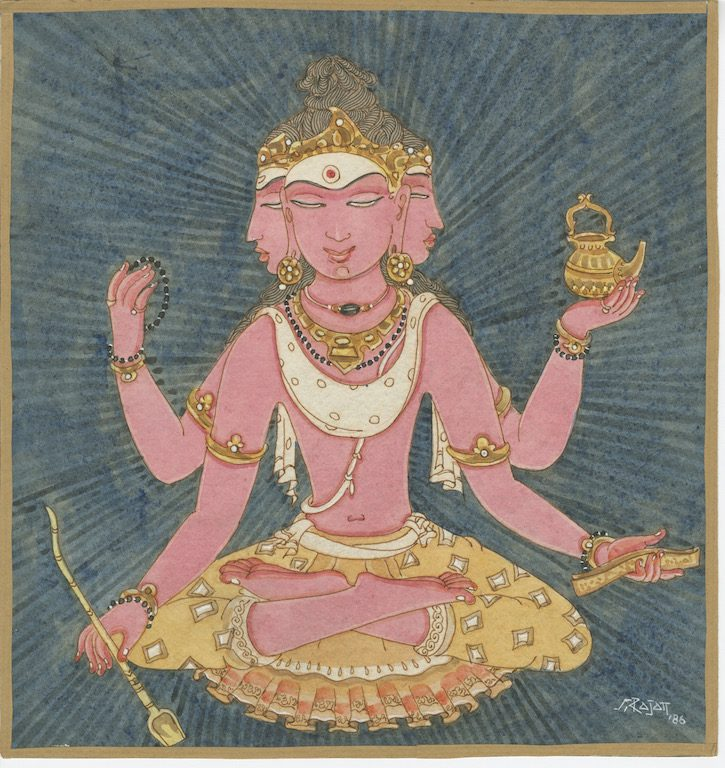
\includegraphics[width=0.5\textwidth]{pics/Brahma.png}
\caption{ Lord Brahma}
 \end{figure}

 

\begin{enumerate}

\item[ ] 1. Brahma or Prajapati, the cosmic creator. This tithi is good for initiating all ventures and for all sacraments and spiritual actions. It is particularly good for planning things, but not so much for actually starting or doing things. The new Moon still casts a shadow on this day.

Prajapati is also the ruler of Rohini (mid-Taurus), the most favorable of the Nakshatras. This tithi, like Rohini, is very good for promoting all positive actions in the initial phase of things. On this tithi one should set forth ones plans for the month.

 

\item[ ] 2. Vidhatar, the cosmic ordainer. This deity is like Brahma but more concerned with establishing structure and order. Whereas the first tithi is good for plans, for planting the seeds of things, this tithi is better for establishing the broader scope of our endeavors.

It has an energy similar to Abijit, also ruled by Vidhatar, a very favorable Nakshatra for giving great victory and high achievement.

 

\item[ ] 3. Vishnu, the cosmic preserver. This tithi is thus good for activities that are meant to be enduring. It is good for bringing things to a high level of development and recognition.

It has an energy similar to Shravana (mid-Capricorn), ruled by Vishnu, which is good for communication, public and teaching ventures.

 

\item[ ] 4. Yama, the God of death and discipline. This tithi is thus unfavorable except for harsh actions and self-discipline.

It has an energy similar to Bharani, also ruled by Yama, and brings karmic retribution.

 

\item[ ] 5. The Moon, Soma. This tithi is favorable for most activities, particularly those involving women, the mother and the emotional nature, which relate to the Moon. It is good for preparing or taking herbal medicines and for natural healing therapies of both body and mind. It is favorable for devotional meditation.

It has an energy similar to Mrigashiras (Orion, late Taurus/early Gemini), also ruled by Soma.

 

\item[ ] 6. Agni, Fire or Skanda, the War God

Ruled by fire, this tithi is good for harsh or fiery actions: Surgery, overcoming enemies, disciplining our physical nature or organizing our material resources.

It has an energy similar to Krittika (the Pleiades, early Taurus), also ruled by Agni.

 

\item[ ] 7. Indra: Deity of Self-power and Transcendence

This tithi is good for actions aimed at establishing independence, for personal gains and for self-development. It can give great success but requires will and motivation.

It has an energy similar to Jyeshta (late Scorpio), ruled by Indra, but is more favorable.

 

\item[ ] 8. The Vasus: Gods of Splendor

It has an energy similar to Dhanishta, ruled by the Vasus. It gives success and splendor but with a tendency toward excess, overdevelopment and diffusion of energies.

 

\item[ ] 9. The Serpent

It has an energy similar to Uttara Bhadra ruled by Ahir Budhnya and hence is to be avoided. It also inclines toward excess and possible deception.

 

\item[ ] 10. Dharma or Brihaspati, God of Religion and Truth

This tithi is favorable for all dharmic and spiritual actions, for rituals, meditation, and for all sacraments and positive actions in life.

It has an energy similar to Pushya (mid-Cancer), also ruled by Brihaspati, which gives the ability to promote all positive ventures.

 

\item[ ] 11. Rudra or Shiva, Deity of Destruction

This tithi is very strong and can give success and transformation but its energy can be difficult to deal with, like the fierce God Rudra. It has an energy similar to Ardra (mid-Gemini), also ruled by Rudra. Yet it is also used for the worship of Vishnu.

 

\item[ ] 12. The Sun (Aditya or Savitar):

This tithi is very auspicious for creative and spiritual actions, particularly for creative work and learning.

It has an energy similar to Hasta (mid-Virgo), also ruled by Savitar.

 

\item[ ] 13. God of Love and Charm (Bhaga):
This tithi is favorable for matters of pleasure, enjoyment, recreation, friendship, social gains, charm, charisma and dealing with the mass media.

It has an energy similar to Purva Phalguni (mid-Leo), also ruled by Bhaga.

 

\item[ ] 14. Strife

This tithi causes conflict and misunderstanding. It is only good for harsh actions like administering drugs or performing surgery, or for black magic.

It has an energy similar to Ashlesha (late Cancer), which can give deception.

 

\item[ ] 15. Full Moon: Universal Gods (Vishve Devas)

This tithi is good for worshipping the Divine, for cosmic action and for promoting the future.

It has an energy similar to Uttarashadha (late Sagittarius), ruled by the Universal Gods.

 

\item[ ] 15. New Moon – the Ancestors

This tithi is good for worshipping the Ancestors, or dealing with ones past.

It has an energy similar to Magha (early Leo), ruled by the Ancestors. It is better for self-examination and for clearing up the past.

The first half of the lunar month is better for spiritual actions and for initiating new activities. The second half is better for personal, social or family matters and for finishing off actions already started.

 

\subsubsection{TITHIS AND PLANETARY ASPECTS}

Each tithi covers 12 degrees of arc between the Sun and Moon. The purna tithis roughly parallel 60, 120 and 180 degree aspects between the Sun or Moon, or trines, benefic aspects in Western astrology. The rikta tithis roughly parallel 45º, 90º and 135º or square and semi-square aspects, malefic aspects in Western astrology.

 

\subsubsection{III. THE DAYS OF THE WEEK}
 

Each day of the week has its characteristic quality based upon the nature of the planet that rules it. Again we must note that the Vedic day begins at sunrise. The nature of the day is the easiest factor to consider, as it requires neither an ephemeris nor a Panchanga. It is usually the first factor that we should consider, and the basis for determining the Nakshatra and Tithi. If we choose an auspicious day for our actions, we have already taken a significant step in protecting them.

 

\subsubsubsection{BENEFIC AND MALEFIC DAYS}

\paragraph{}Days ruled by benefic planets – Monday, Wednesday, Thursday and Friday – Moon, Mercury, Jupiter and Venus – are good for most actions. 
\paragraph{}Thursday and Friday are the best, as Jupiter and Venus are the most auspicious planets.
\paragraph{}Days ruled by malefic planets – Sunday, Tuesday and Saturday – Sun, Mars, and Saturn – have some unfavorability. 
\paragraph{}Tuesday and Saturday are worse in this respect, as their lords are most malefic.


\subsubsubsection{INDICATIONS OF DAYS OF THE WEEK}
 

SUNDAY

Favorable for rituals, meditation, self-knowledge, gains in career or status, receiving honors, honoring tradition, authorities, parents or gurus, worship of the Divine Father (Shiva or Vishnu). Unfavorable for marriage, sexual activity or conception. Not generally useful for business ventures. Not a good day for outward expansion as much as inner examination and for establishing personal intentions and goals to be realized during the week.

 

MONDAY

Favorable for affairs relating to the public or society, for gaining popularity, for relating to women or to the mother, including worship of the Divine Mother, for friends, family and household matters in general. It is good for marriage, sexual activity and conception of children, medical treatment (the Moon is a nurse), rituals, particularly of a devotional nature, and for contemplation and meditation. Can bring financial or business gains through friends and social contact.

 

TUESDAY

Good for physical activity, sports and competitive ventures (but care must be taken not to act recklessly). It is important that we use the restless Mars energy of this day and do not allow it to become bottled up inside ourselves. It is good for developing a warrior energy, and for worshipping Lord Skanda, the Divine warrior (or Rudra, the wrathful form of Shiva, and Candi or Durga, the wrathful form of the Goddess). Also useful for mechanical work, fixing things, for research, mathematical studies, and scientific pursuits.

Tuesday is more favorable in the afternoon than in the morning. Unfavorable for marriage or sexual activity. Generally not good for travel, for legal affairs, for relationship and human issues requiring tact or sensitivity.

 

WEDNESDAY

Good for talking, writing, learning, study, teaching, educational activities, meditation and the development of discrimination. Good for business, commerce, and career gains, communication ventures, making money, marriage and sexual activity. Good for all healing practices, particularly using herbs, and the making of medicines. Also good for healing the mind and all psychological studies. A good day for the worship of Lord Vishnu. Yet more a day for creating the theoretical background for our projects than for trying to initiate anything lasting.

 

THURSDAY

The most favorable day of the week generally for all good actions, including religious rituals, ceremonies, meditation, study and worship of the Divine, the guru or traditions. Good for financial gain, speculative ventures, career advancement, and for enjoyment and social interaction. Good for healing practices in general, exercise of all types, reconciliation, and for giving gifts. Excellent for legal matters. Favorable for marriage, sexual activity, or conception of children. Also good for the affairs of children. The best day for initiating expansive ventures that we hope will endure. Good for worshipping Lord Ganesha.

 

FRIDAY

Good for artistic ventures, decorations and ornaments, business ventures, purchasing vehicles, buying gems, clothes, or other precious items, for affairs relative to women (marriage, sexual activity, romance), enjoyment and entertainment. Also good for devotional practices or study of the occult, particularly for the worship of the Divine Mother, especially in her blissful form (Lalita).

 

SATURDAY

Unfavorable for most social or business matters, as it usually brings loss or opposition, but good for acquiring fixed property and for doing service work. Not good for health, marriage, or for sexual activity, but good for retreat, study, meditation and relaxation. Also good for self-discipline, yoga, fasting and ascetic practices. A good day to spend time alone. Good for worshipping the dark or wrathful forms of the Divine, like the terrible forms of Shiva (like Bhairava) and his consort (like Kali).

Our cultural tendency is to escape the influence of Saturn on Saturday by turning it into a day of self-indulgence but this is not wise, as it keeps our lives out of the control of our deeper nature and spiritual intent. Hence, Saturday is perhaps the most important day of the week for structuring our time wisely.

 

\subsubsection{NOTES ON THE DAYS}

 

We must remember that these are only general indications. The position of the planet on that day must be considered as well. For example, if Mercury is with Saturn and Rahu, Wednesday may cause loss and difficulties with communication and business.

 

The effects of the days of the week on an individuals life varies according to the place and strength of the planet within the individuals birth chart. For example, if a person has a strong Mars as a Raja Yoga Karaka, Tuesday would be very favorable for work, career, or starting new ventures.

 

\subsubsection{COMBINING THE DAY, TITHI AND NAKSHATRA}

It is best to combine favorable days, Tithis and Nakshatras for the best possible results. When a favorable day of the week, like Thursday or Friday, is under a favorable Tithi, like the fifth or the tenth, it is a good day for auspicious actions. If, in addition, the Moon is in a favorable Nakshatra – like Pushya, Punarvasu, Rohini, Mrigashiras, Revati, Uttara Phalguni, Uttara Bhadra or Chitra – then the results are quite excellent.

 

When such a good day is under a favorable Tithi for meditation, like the ninth, fourteenth or fifteenth, then it becomes very strong for that. If, in addition, the Moon is in a Nakshatra favorable for worship, which varies relative to the type of deity or the type of worship involved, the results will also be favorable.

 

\subsection{IV. KARANAS}


Each Tithi is divided into two Karanas. Karana means “instrument”. The Karanas help give us the means to fulfill our actions. These are named according to different animals. In total there are eleven Karanas.

 

\subsubsection{KARANAS}

 
\begin{center}
\begin{tabular}{ l l l}
1.  LION (Bava)&	2,  9, 16, 23, 30, 37, 45, 51             \\
2.  LEOPARD (Balava)	&3, 10, 17, 24, 31, 38, 46, 52            \\
1.    PIG (Kaulava)	&4, 11, 18, 25, 32, 39, 47, 53            \\
2.    DONKEY (Taitula)	&5, 12, 19, 26, 33, 40, 48, 54            \\
3.    ELEPHANT (Garija)	&6, 13, 20, 27, 34, 41, 49, 55            \\
4.    COW (Vanija)	&7, 14, 21, 28, 35, 42, 50, 56            \\
5.    VISHTI	&8, 15, 22, 29, 36, 43, 51, 57            \\
6.    PULLU (Shakuna)	&58            \\
7.    CATTLE (Chatuspada)	&59            \\
8.    SNAKE (Naga)	&60            \\
9.    WORM (Kimstughna)	&1            \\
\end{tabular}
\end{center}

 
\begin{enumerate}

\item[*] The first one and last three Karanas are fixed in nature. They relate to the time of the new Moon and show the enduring factor of the Moons power.

 

\item[*] The remaining fifty-six Karanas are said to be mutable in nature. They show the fluctuations of the lunar force.

 

\item[*] The fixed Karanas and the Vishti Karanas are considered to be generally unfavorable in nature and actions should not be done during them.

 

\item[*] The fixed Karanas occur during unfavorable Tithis anyway and are generally rejected on that account. They relate to the latter half of the fourteenth day of the waning Moon, the day of the new Moon, and the first half of the day after the new Moon. Hence, the first half of the first day of the waxing Moon is more unfavorable than the second half. By this system, we can understand why the new Moon, though technically a Purna or full Tithi, is unfavorable. Both of its Karanas are negative.

 

\item[*] The Fixed Karanas (58, 59, 60, 1) and, of the Mutable class, those of the Vishti group (8, 15, 22, 29, 36, 43, 50, 57) are considered to be generally unfavourable and inauspicious in nature, therefore, the performance of any kind of action should be avoided under them.

 

\item[*] The Fixed Karanas, occurring once a (lunar) month as a transition between the two halves (Pakshas) of the Moon, cover a two-day time period, in lunar terms, (four consecutive half-days, or two Tithis).

 

\item[*] For the remaining period of time, the Karanas of Vishti (and of the other groups) occur in alternation eight times each in a (lunar) month, on every seventh (lunar) half-day (8 x 7 = 56).

 

\item[*] Vishti Karana occurs in the bright half of the Moon in the first half of the 4th Tithi (which is generally rejected as unfavorable anyway), the first half of the 8th Tithi (also generally rejected), the second half of the 11th Tithi, and the first half of the full Moon Tithi. During the dark half of the Moon, it occurs on the second half of the 3rd Tithi, the first half of the 7th Tithi, the second half of the 10th Tithi, and the first half of the 14th Tithi (also generally rejected).

 

\item[*] The Karanas of the lion are good for starting ventures of an enduring nature, those of the donkey are good for marriage.

 \end{enumerate}

\subsubsection{INDICATIONS OF KARANAS}

 

Below are some typical classical indications of the Karanas mainly for birth but also for action. They are delineated briefly, as in themselves they are not that important.

 
\begin{center}
\begin{tabular}{ l l l}
1. BAVA	&Youthful, childish, valiant                         \\
2. BALAVA	&Modest, careful in conduct, respected                        \\
3. KAULAVA	&Impressive, active, dramatic                        \\
4. TAITULA	&Skillful in speech and action, able to influence                        \\
5. GARIJA	&Powerful, able to overcome opposition                        \\
6. VARIJA	&Clever, passionate, may be lacking in self-control                        \\
7. VISHTI	&Gives opposition, acts contrary to normal order, culpable, self-reliant, honored by his followers                        \\
8. SHAKUNA	&Able to read events, psychic perception, intelligence, prosperity                        \\
9. CHATUSPADA	&Many obstacles, yet many possibilities, comprehensive                        \\
10. NAGA	&Ambitious, powerful, dangerous                        \\
11. KIMSTUGHNA	&Dependent, changeable, superficial, easy going                        \\
\end{tabular}
\end{center}
 

 

\subsection{V. PANCHANGA YOGAS}
 

The term Yoga has several usages in Vedic Astrology. Here it is used relative to Muhurta or Electional Astrology. Like the Nakshatras, each Yoga relates to a 13º 20 section of the zodiac. Yet it is calculated differently. Below we present how to calculate the Yogas. This material, however, is not important to memorize, as most of the time we will merely look the Yogas up in the almanac.

 
\begin{enumerate} 
\item[] To calculate the Yoga, add the longitudes of the Sun and the Moon and divide the amount by 800 (the number of minutes in 13°20).

 

\item[] For example, if the Moon is at 14° 20 Gemini, its longitude from the point 0 Aries would be 74° 20. If the Sun is at 20° 40 Sagittarius, its longitude would be 260° 30.

 

\item[] Adding these together, 74°20 plus 260°40 we would get 334° 50. If we get a number higher than 360, we should subtract 360 from it.

 

\item[] This we then turn into minutes by multiplying the degrees by 60, which would be 20,040 plus 50 for the minutes or 20,090.

 

\item[] We then divide this amount by 800, which gives us 25.1125. This places us in the twenty-sixth yoga – Brahma yoga – as the twenty-fifth has already finished.

 

\item[] To determine when a particular yoga ends, multiply the remainder by 24. In the above example 24 x .1125 is 2.7 or two houses and forty-two minutes from the particular time in question.

 \end{enumerate}

\subsubsection{INDICATIONS OF YOGAS}
 

Below are typical indications of Yogas both for birth charts and for the purposes of astrological forecasting.

 
\begin{center}
\begin{tabular}{ l l l}
1.    VISHKAMBHA*	&Overcomes obstacles, gains wealth and property                                \\
2.    PRITI*	&Easily influenced by attractive objects                               \\
3.    AYUSHMAN	&Good for health and longevity                               \\
4.    SAUBHAGYA	&Gives happiness, is auspicious for action                               \\
5.    SOBHANA	&Gives beauty but also sensuality                               \\
6.    ATIGANDA*	&Destructive and deceptive tendency, clever                               \\
7.    SUKARMA	&Good for action, work and accomplishment                               \\
8.    DHRITI*	&Dominates and controls other people                               \\
9.    SHULA*	&Gives anger, conflict and pain                               \\
10. GANDA*	&Gives attachments and addictions                               \\
11. VRIDDHI	&Gives wisdom, speech capacity and increase                               \\
12. DHRUVA	&Gives stability, firmness and wealth                               \\
13. VYAGHATA*	&Dangerous and wrathful, can bring injury                               \\
14. HARSHANA	&Exhilarating, gives joy, fame and wisdom                               \\
15. VAJRA*	&Gives will, power, energy and motivation                               \\
16. SIDDHI	&Gives success and protection                               \\
17. VYATIPATHA*	&Deceptive, unclear, moving in many directions                               \\
18. VARIYAN*	&Causes one to seek gain, can give greed, ambition                               \\
19. PARIGHA*	&Inimical but wealthy and successful                               \\
20. SHIVA 	&Auspicious, peaceful, intelligent, loved                               \\
21. SIDDHA	&Successful, virtuous, adept, skillful                               \\
22. SADHYA	&Righteous (virtuous), able to accomplish goals                               \\
23. SHUBHA	&Gives beauty and wealth but may give sensuality                               \\
24. SHUKLA	&Gives intelligence, powers of speech, is virtuous but changeable in mind and difficult to please                               \\
25. BRAHMA	&Gives wisdom, good judgment, honor, secret wealth                               \\
26. AINDRA	&Gives comprehensive intellect, beneficence, wealth, power, honor, prestige                               \\
27. VAIDHRITI*	&Firm, powerful, wealthy but obstinate and inflexible                               \\
\end{tabular}
\end{center}
 

*less favorable

 

\begin{enumerate} 
\item[] Of these Yogas, the first, sixth, ninth, tenth, fifteenth, seventeenth and twenty-seventh are inauspicious.
\item[] The twenty-first, twenty-fifth and twenty-sixth are particularly auspicious.
\item[] All other remaining Yogas are considered favourable, particularly 21 (Siddha), 25 (Brahma), and 26 (Aindra), under which all auspicious undertakings are permitted.
 

Main  Inauspicious  Yogas

 
\begin{center}
\begin{tabular}{ l l l}
Yoga	Sanskrit  &Name	Meaning	&Time  Period  To  Be  Avoided                               \\
1	Vishkambha	&Pot filled with poison	&First 3 Ghatis (1 hour  and 12 minutes)                               \\
6	Ati-Ganda	&Very strong knot (obstacle)	&First 6 Ghatis (2 hours and 24 minutes)                               \\
9	Shula	&Sharp or pointed weapon	&First 5 Ghatis (2 hours)                               \\
10	Ganda	&Knot (hindrance)	&First 6 Ghatis (2 hours and 24 minutes)                               \\
13	Vyaghata	&Striking against (obstacle)	&First 9 Ghatis (3 hours and 36 minutes)                               \\
15	Vajra	Thunderbolt, lightening	&First 3 Ghatis (1 hour  and 12 minutes)                               \\
17	Vyatipata	&Destruction	 &60 Ghatis (Whole time period)                               \\
19	Parigha	&Iron bar / club	&30 Ghatis (First half of Yoga)                               \\
27	Vaidhriti	&Division	&60 Ghatis (Whole time period)                               \\
 \end{tabular}
\end{center}

\subsubsection{USING KARANA AND YOGA}

Once we have determined a favorable Day, Tithi and Nakshatra, we should check to see if an unfavorable Yoga and Karana are in existence that could cause obstruction. If this is not the case, the outcome becomes more favorable. If it is the case, we may look to a part of the day when the negative Yogas and Karanas are not in operation, or we can look to another favorable day, Tithi and Nakshatra that do not have such a negative condition.

 

There is a part of this system which delineates specific Tithis coinciding with particular days of the week as being auspicious or inauspicious. Certain combinations of weekdays and lunar days, Varas and Tithis, give rise to certain qualities during the time period in question, according to the integration of the individual qualities of these two time factors.

 

Siddha Tithi  (Auspicious Tithis)

 
\begin{center}
\begin{tabular}{ l l l}
Tithi  Group	&Tithis	&Vara                                     \\
Nanda	&1,  6,  11&	Friday                              \\
Bhadra	&2,  7,  12	&Wednesday                              \\
Jaya	&3,  8,  13	&Tuesday                              \\
Rikta&	4,  9,  14	&Saturday                              \\
Purna	&5, 10, 15	&Thursday                              \\
 \end{tabular}
\end{center}

Dagdha Tithi  (Inauspicious Tithis)

 
\begin{center}
\begin{tabular}{ l l l}
Tithi  Group	&Vara                              \\
Nanda	&Sunday, Tuesday                              \\

Bhadra	&Monday, Friday                              \\

Jaya	&Wednesday                              \\
Rikta	&Thursday                              \\
Purna	&Saturday                              \\
  \end{tabular}
\end{center}

Krakacha  Tithi  (Inauspicious Tithis)

(Tithi + Vara = 13)

 
\begin{center}
\begin{tabular}{ l l l}
Tithi	&Vara \\
12 Dwadashi	&1 Sunday                             \\
11 Ekadashi	&2 Monday                             \\
10 Dashami	&3 Tuesday                             \\
  9 Navami	&4 Wednesday                             \\
  8 Ashtami	&5 Thursday                             \\
  7 Saptami	&6 Friday                             \\
  6 Shashti	&7 Saturday                             \\
   \end{tabular}
\end{center}

 
\subsubsection{ADDITIONAL FACTORS BEYOND THE PRIMARY FIVE}
 

There are several additional factors to consider beyond the usual five of the Panchanga, which overlap with them to some degree.

 

\subsubsection{ADDITIONAL FACTORS RELATIVE TO THE SUN}
 

There are some incidental factors relative to the Sun that should be considered for the timing of actions.

 

\subsubsection{THE SUN’S MOVEMENT INTO NEW SIGNS – SANKRANTI}

The Sun’s movement into new signs of the zodiac, called Sankranti, is also a time period that is not favorable for actions. It is similar to the Western idea of the Moon being void of course and hence unfavorable when it crosses between signs. It is mainly the period of about six hours before and after changing signs that is inauspicious, the last fifteen minutes or quarter of a degree of one sign and the first fifteen minutes of another.

 

When other planets are in the last or first degree of a sign, this can also cause difficulties.

 

\subsubsection{EQUINOCTIAL AND SOLSTICE POINTS}

The days of the equinoxes and solstices are additional important transitional periods. Hence, they are more favorable for rituals and meditation than for ordinary activities. Most important perhaps is the day of the winter solstice as it allows us to bring in a spiritual energy for the whole year.

 

Like transitional points of sunrise and sunset, the solstices and equinoxes are points at which the mind can more easily become still and the Prana or vital energy can enter the central channel for inner transformation. Hence, these times are important for spiritual rather than ordinary actions.

 

\subsubsection{THE NORTHERN AND SOUTHERN COURSES OF THE SUN}

Actions are best done during the northern course of the Sun (Uttarayana), the period between the winter and the summer solstices (December 22—June 21). This is the best time for such things as marriages, initiations, or even for death (it is best to die at the winter solstice according to Vedic thought).

 

For actions done in the southern course of the Sun, they are best if done during the bright half of the Moon.

 

The northern course of the Sun, as we noted in the section of the course on chakras, relates to the movement of the Prana up the spine. Hence, it is also better for spiritual practices.

 

\subsubsection{ECLIPSES}

Eclipses are important points of energy transformation, and perhaps the most important transitional periods of all. They bring the energy into the central channel and allow the mind to be still, withdrawing it from its ordinary outward actions. Hence, they are also very favorable for rituals and meditation but not for ordinary activities.

 

Lunar eclipses are important times for purification and negation of the mind. Solar eclipses are important times for self-knowledge and transcendence of the ego.

 

\subsubsection{GANDANTA MOON}
The Moon located in the first navamsha (3º 20) of fire signs or the last quarter of water signs is inauspicous for actions and dangerous for the birth of children. This position is the first quarter of Ashwini, Magha and Mula Nakshatras and the last of Revati, Aslesha and Jyeshta Nakshatras.

 

Jyeshta-Mula or Scorpio-Sagittarius Gandanta is considered to be the worst. Aslesha-Magha or Cancer-Leo Gandanta is second. Revati-Ashwini or Pisces-Aries is not always so bad.

 

The same positions are difficult for other planets but only in the first and last degrees of the respective signs, not through the entire 3º 20 section. The full Gandanta arc of 3º 20 applies only to the Moon as it is a fast-moving planet.

 

\subsubsection{LUNAR MONTHS}
In India, a lunar calendar is employed from new Moon to new Moon, named after the Nakshatra in which the Moon becomes full in during the month. The twelve Hindu months are:

 
\begin{center}
\begin{tabular}{ l l l}
Ashwin – October	&Karttika – November                              \\
Margashirsa – December	&Pushya – January                             \\
Magha – February	&Phalguni – March                             \\
Caitra – April	&Vaishakha – May                             \\
Jyeshta – June	&Ashadha – July                             \\
Shravana – August	&Bhadrapada – September                             \\
   \end{tabular}
\end{center} 

As these months depend upon the Moon, they vary slightly every year and hence their equivalence to various Western months is very approximate. Again, an almanac is needed for determining them. Every 2½ years an additional or intercalary month has been added, as the lunar year of twelve months falls eleven days short of the solar year of 365 days.

 

The different lunar months have their own characteristics and importance. Various days within them relate to holy days among the Hindus and Buddhists. This matter has its complexity and it is our intention only to introduce it here.

 

Generally, the months comprising the northern course of the Sun (Margashirsha to Jyeshta) are better than those under the southern course (Ashadha to Karttika).

 

The month of Magha is generally not favorable for putting on gems, installing altars or forms of deities, or other religious and spiritual issues. The months of Karttika and Mrigashiras are particularly favorable for spiritual practices and rituals. Different Hindu and Buddhist deities have their special days in different months, like Shiva Ratri in February, the nine days of Durga in October, the sacred day of the Buddha in Vaishakha, or the birth day of Krishna in August. These are regulated according to the lunar calendar.

However, the months are a secondary consideration, as many actions must be performed every month.

 

\subsubsection{THE PLACE OF ASTROLOGICAL FORECASTING}

Naturally, we dont always have the time to examine all such astrological factors in detail before initiating all actions, and astrology cannot substitute for our own power of judgment. In the modern world, we cannot always modify these factors either. For example, we cannot always get airplane tickets at the most auspicious times for travel. And, just because a day is favorable for accumulating wealth does not mean that it is right for us to do so. We must always look back to the dharma of the person to determine which of these favorable potentials is best for them. In this regard, it is more important that we do what is best for us, rather than do what is best for the particular day involved, though it is ideal to be able to combine both together to some degree. If we focus on the spiritual life, for example, many of these outer potentials lose their attraction for us.

 

As an astrologer, astrological forecasting may not be our primary interest but we should at least be acquainted with the subject or we cannot be said to be truly aware of the complete scope of Vedic Astrology.

 

For further study, we recommend the Kala Prakashika, translation by N.P. Subramania Iyer. Yet we should note that, owing to changes in time and culture, the whole system of Astrological Forecasting requires perhaps more readjustment than the reading of birth charts. Much of the traditional information on the subject, reflecting the customs of medieval India, may not be of relevance for us today.

 


\subsubsection{SUPPLEMENT
LUNAR MONTHS AND SACRED TITHIS OF THE HINDU CALENDAR}
 

The following days are good for various planets and various actions even apart from the usual Tithi and Nakshatra indications. As these lunar months vary every year, you must check the yearly Panchanga to find out which exact days of the Western solar calendar they correspond to. Actions done on special days are much more powerful. This extends to astrological remedial measures.

(Key:  * sacred days    ** days good for all actions, Shukla is waxing Moon, Krishna or K. is waning Moon, month indications begin with waxing Moon)

 

Chaitra – April

 
\begin{enumerate} 
\item[] **Pratipat – Astronomical new year  — all
\item[] Panchami – Matsya  Jayanti — Ketu
\item[] Ashtami – Durga — Rahu
\item[] *Navami – Rama Jayanti — Sun
\item[] Trayodashi – Mahavira (Jaina) Jayanti
\item[] Purnima – Chitragupta/Hanuman Jayanti — Ketu, Mars
\item[] K. Ashtami – Sitala Devi, to counter fevers and diseases — Ketu, Mars
\end{enumerate}
 

Vaishakha – May
\begin{enumerate} 
\item[] **Tritiya – Parshurama Jayanti, Akshayya (Satya Yuga) — all, Venus
\item[] Panchami – Shankaracharya Jayanti
\item[] Saptami – Ganga Devi — Mercury
\item[] Chaturdashi – Nrisimha Jayanti — Mars
\item[] *Purnima – Buddha Purnima, Kurma jayanti — Mercury, Saturn
 \end{enumerate}

Jyeshta – June
\begin{enumerate} 
\item[] Purnima – Savitri, Snana Yatra of Ratha Yatra — Sun
\item[] K. Caturdasha – Savitri
 \end{enumerate}

Ashadha – July
\begin{enumerate} 
\item[] Dvitiya – Rathayatra, Jagannath Puri — Sun
\item[] *Shasti – Skandha — Mars
\item[] Ashtami – Durga Shayana
\item[] Ekadashi – Vishnu Shayana
\item[] *Purnima – Guru Purnima, Vyasa — Jupiter, Mercury
\item[] Shravana – August
\item[] Panchami – Naga Panchami — Rahu, Ketu
\item[] Saptami – TulsiDasha Jayanti
\item[] *Ashtami – Krishna Janmashatami — Moon
\item[] *Purnima – Raksha Bandhana — all malefics
\item[] K. Chaturthi – Ganesha
 \end{enumerate}

Bhadrapada – September
\begin{enumerate} 
\item[] Dvitiya – Balarama Jayanti
\item[] Tritiya – Varaha jayanti
\item[] *Chaturthi – Ganesh Chaturthi – noon — all planets, Jupiter, Ketu
\item[] Panchami – Rishi Panchami — Mercury, Jupiter, Ketu
\item[] Ashtami – Indra Dvaja / Radha Jayanti — Jupiter, Venus
\item[] Dvadashi – Vamana jayanti — Jupiter
\item[] Chaturdashi – Ananta — Rahu, Ketu
\item[] Purnima – Uma Maheshvara Vrata — Sun, Moon
\item[] Krishna  Paksha – Pitripaksha
\item[] K. Trayodashi – Dwapara Yugadi
\item[] Amavasya – Mahalaya — Saturn
 \end{enumerate}

Ashvina – October
\begin{enumerate} 
\item[] Navaratri (nine day festival)
\item[] *Pratipat, *Dvitiya, *Tritiya, *Chaturthi, *Panchami
\item[] *Shashti – Durga Bodhana
\item[] *Saptami – Saraswati — Mercury
\item[] *Ashtami – Durga — Rahu
\item[] *Navami
\item[] **Dashami – Vijay Dashami — Moon, Venus
\item[] Purnima – Sharat Purnima, Lakshmi — Moon, Venus
\item[] K. Trayodashi – Dhanvantari — Mercury
\item[] *K. Caturdashi – Dipavali 1- Naraka Chaturdashi, Kali, Hanuman — Saturn
\item[] *Amavasya – Lakshmi — Moon, Venus
 \end{enumerate}

Karttika – November
\begin{enumerate} 
\item[] **Pratipad – Dipavali, Balipratipat, Bali Puja, religious new year — All
\item[] *Dvitiya – Dipavali, Yama/Yamuna, Vishvakarma
\item[] Shasti – Skanda, Surya – Mars, Sun
\item[] Saptami – Sun
\item[] Navami – Treta Yugadi
\item[] Ekadashi – Vishnu Prabodhini — Mercury, Sun
\item[] Dvadashi – Vishnu Utthana, Tulasi Devi
\item[] Chaturdashi – Vaikuntha Chaturdashi Vrata
\item[] *Purnima – Dipam, Shiva, Skanda — Mars
\item[] K. Ashtami – Bhairavi
\item[] Amavasya – Durga, Kali — Rahu, Saturn
 \end{enumerate}

Margashirsha – December
\begin{enumerate} 
\item[] Chaturthi – Ganapati-Varada — all planets, Jupiter
\item[] *Panchami – Sri/Lakshmi — Moon, Venus
\item[] Shasti – Skanda — Mars
\item[] Ekadashi – Vaikuntha, Gita Pravachana, Gita Jayanti, Vishnu — Sun, Mercury
\item[] Dvadashi – Vaikuntha, Vishnu
\item[] Purnima – Dattatreya, Nataraja Darshana
 \end{enumerate}

Pushya – January
\begin{enumerate} 
\item[] K. Saptami – Vivekananda Jayanti
 \end{enumerate}

Magha – Februrary
\begin{enumerate} 
\item[] *Panchami – Vasanta – Saraswati — Mercury, Moon
\item[] *Saptami – Ratha Saptami – Surya, Vaivasvata Manvantara — Sun
\item[] Ashtami – Bhishma Mahasamadhi
\item[] Ekadashi – Bhima
\item[] Purnima – Snana – Sun
\item[] *K. Chaturdashi – Shiva Ratri — Saturn
\item[] Amavasya – Muni Amavasya/ Kali Yugadi, Mahamela — Saturn
 \end{enumerate}

Phalguna – March
\begin{enumerate} 
\item[] Dvitiya – Ramakrishna Jayanti
\item[] Ashatmi – Sita Jayanti — Venus
\item[] Ekadashi – Amalaki Vrata
\item[] *Purnima – Holi, Prahlada — Venus
\end{enumerate}

All Months
\begin{enumerate} 
\item[] Pratipad, Shukla – For all spiritual actions and initiation
\item[] Chaturthi, particularly Shukla – Ganesh — Jupiter, Ketu
\item[] Panchami, Shulka – The Goddess in her benefic forms, Lakshmi, Saraswati — Moon, Venus
\item[] Shasti, particularly Shukla – Skanda — Mars
\item[] Ashtami, Shukla – Devi – Moon, Venus, Rahu
\item[] Dashami, Shukla – Good for all planets
\item[] Ekadashi – Vishnu, particularly Shukla — Sun, Mercury, Also good for fasting
\item[] Trayodashi, Shukla — Pradosha, Shiva
\item[] Purnima – For meditation
\item[] K. Chaturdashi – Shiva, Kali, Masa Amavasya — Saturn
 \end{enumerate}

Other Important Dates
\begin{enumerate} 
\item[] Also Sankrantis or Sun changing signs, particularly Capricorn and Cancer
\item[] Solstices, equinoxes, and eclipses
\end{enumerate}